\documentclass[twoside]{book}

% Packages required by doxygen
\usepackage{calc}
\usepackage{doxygen}
\usepackage{graphicx}
\usepackage[utf8]{inputenc}
\usepackage{makeidx}
\usepackage{multicol}
\usepackage{multirow}
\usepackage{fixltx2e}
\PassOptionsToPackage{warn}{textcomp}
\usepackage{textcomp}
\usepackage[nointegrals]{wasysym}
\usepackage[table]{xcolor}

% Font selection
\usepackage[T1]{fontenc}
\usepackage{mathptmx}
\usepackage[scaled=.90]{helvet}
\usepackage{courier}
\usepackage{amssymb}
\usepackage{sectsty}
\renewcommand{\familydefault}{\sfdefault}
\allsectionsfont{%
  \fontseries{bc}\selectfont%
  \color{darkgray}%
}
\renewcommand{\DoxyLabelFont}{%
  \fontseries{bc}\selectfont%
  \color{darkgray}%
}
\newcommand{\+}{\discretionary{\mbox{\scriptsize$\hookleftarrow$}}{}{}}

% Page & text layout
\usepackage{geometry}
\geometry{%
  a4paper,%
  top=2.5cm,%
  bottom=2.5cm,%
  left=2.5cm,%
  right=2.5cm%
}
\tolerance=750
\hfuzz=15pt
\hbadness=750
\setlength{\emergencystretch}{15pt}
\setlength{\parindent}{0cm}
\setlength{\parskip}{0.2cm}
\makeatletter
\renewcommand{\paragraph}{%
  \@startsection{paragraph}{4}{0ex}{-1.0ex}{1.0ex}{%
    \normalfont\normalsize\bfseries\SS@parafont%
  }%
}
\renewcommand{\subparagraph}{%
  \@startsection{subparagraph}{5}{0ex}{-1.0ex}{1.0ex}{%
    \normalfont\normalsize\bfseries\SS@subparafont%
  }%
}
\makeatother

% Headers & footers
\usepackage{fancyhdr}
\pagestyle{fancyplain}
\fancyhead[LE]{\fancyplain{}{\bfseries\thepage}}
\fancyhead[CE]{\fancyplain{}{}}
\fancyhead[RE]{\fancyplain{}{\bfseries\leftmark}}
\fancyhead[LO]{\fancyplain{}{\bfseries\rightmark}}
\fancyhead[CO]{\fancyplain{}{}}
\fancyhead[RO]{\fancyplain{}{\bfseries\thepage}}
\fancyfoot[LE]{\fancyplain{}{}}
\fancyfoot[CE]{\fancyplain{}{}}
\fancyfoot[RE]{\fancyplain{}{\bfseries\scriptsize Generated on Fri Dec 5 2014 00\+:39\+:08 for My Project by Doxygen }}
\fancyfoot[LO]{\fancyplain{}{\bfseries\scriptsize Generated on Fri Dec 5 2014 00\+:39\+:08 for My Project by Doxygen }}
\fancyfoot[CO]{\fancyplain{}{}}
\fancyfoot[RO]{\fancyplain{}{}}
\renewcommand{\footrulewidth}{0.4pt}
\renewcommand{\chaptermark}[1]{%
  \markboth{#1}{}%
}
\renewcommand{\sectionmark}[1]{%
  \markright{\thesection\ #1}%
}

% Indices & bibliography
\usepackage{natbib}
\usepackage[titles]{tocloft}
\setcounter{tocdepth}{3}
\setcounter{secnumdepth}{5}
\makeindex

% Hyperlinks (required, but should be loaded last)
\usepackage{ifpdf}
\ifpdf
  \usepackage[pdftex,pagebackref=true]{hyperref}
\else
  \usepackage[ps2pdf,pagebackref=true]{hyperref}
\fi
\hypersetup{%
  colorlinks=true,%
  linkcolor=blue,%
  citecolor=blue,%
  unicode%
}

% Custom commands
\newcommand{\clearemptydoublepage}{%
  \newpage{\pagestyle{empty}\cleardoublepage}%
}


%===== C O N T E N T S =====

\begin{document}

% Titlepage & ToC
\hypersetup{pageanchor=false,
             bookmarks=true,
             bookmarksnumbered=true,
             pdfencoding=unicode
            }
\pagenumbering{roman}
\begin{titlepage}
\vspace*{7cm}
\begin{center}%
{\Large My Project }\\
\vspace*{1cm}
{\large Generated by Doxygen 1.8.7}\\
\vspace*{0.5cm}
{\small Fri Dec 5 2014 00:39:08}\\
\end{center}
\end{titlepage}
\clearemptydoublepage
\tableofcontents
\clearemptydoublepage
\pagenumbering{arabic}
\hypersetup{pageanchor=true}

%--- Begin generated contents ---
\chapter{Hierarchical Index}
\section{Class Hierarchy}
This inheritance list is sorted roughly, but not completely, alphabetically\+:\begin{DoxyCompactList}
\item C\+Elevator\+Controller\begin{DoxyCompactList}
\item \contentsline{section}{C\+Controller}{\pageref{class_c_controller}}{}
\end{DoxyCompactList}
\item \contentsline{section}{C\+Floor}{\pageref{class_c_floor}}{}
\item C\+Frame\+Wnd\begin{DoxyCompactList}
\item \contentsline{section}{C\+Main\+Frame}{\pageref{class_c_main_frame}}{}
\end{DoxyCompactList}
\end{DoxyCompactList}

\chapter{Class Index}
\section{Class List}
Here are the classes, structs, unions and interfaces with brief descriptions\+:\begin{DoxyCompactList}
\item\contentsline{section}{\hyperlink{class_c_about_dlg}{C\+About\+Dlg} \\*The About dialog box }{\pageref{class_c_about_dlg}}{}
\item\contentsline{section}{\hyperlink{class_c_actor}{C\+Actor} \\*Class for actors in our drawings }{\pageref{class_c_actor}}{}
\item\contentsline{section}{\hyperlink{class_c_actor_factory}{C\+Actor\+Factory} \\*Abstract base class for actor factories }{\pageref{class_c_actor_factory}}{}
\item\contentsline{section}{\hyperlink{class_c_butch_factory}{C\+Butch\+Factory} \\*Creates a new actor -\/ Butch }{\pageref{class_c_butch_factory}}{}
\item\contentsline{section}{\hyperlink{class_c_canadian_experience_app}{C\+Canadian\+Experience\+App} \\*Program application class }{\pageref{class_c_canadian_experience_app}}{}
\item\contentsline{section}{\hyperlink{class_c_drawable}{C\+Drawable} \\*Abstract base class for drawable elements of our picture }{\pageref{class_c_drawable}}{}
\item\contentsline{section}{\hyperlink{class_c_harold_factory}{C\+Harold\+Factory} \\*Factory class that builds the Harold character }{\pageref{class_c_harold_factory}}{}
\item\contentsline{section}{\hyperlink{class_c_head_top}{C\+Head\+Top} \\*A class for representing the top of an actor's head }{\pageref{class_c_head_top}}{}
\item\contentsline{section}{\hyperlink{class_c_image_drawable}{C\+Image\+Drawable} \\*Class representing an image drawable (not polygon) }{\pageref{class_c_image_drawable}}{}
\item\contentsline{section}{\hyperlink{class_c_main_frame}{C\+Main\+Frame} \\*Program main frame }{\pageref{class_c_main_frame}}{}
\item\contentsline{section}{\hyperlink{class_c_picture}{C\+Picture} \\*The picture we are drawing }{\pageref{class_c_picture}}{}
\item\contentsline{section}{\hyperlink{class_c_picture_factory}{C\+Picture\+Factory} \\*A factory class that builds our picture }{\pageref{class_c_picture_factory}}{}
\item\contentsline{section}{\hyperlink{class_c_picture_observer}{C\+Picture\+Observer} \\*Observer base class for a picture }{\pageref{class_c_picture_observer}}{}
\item\contentsline{section}{\hyperlink{class_c_poly_drawable}{C\+Poly\+Drawable} \\*A drawable based on polygon images }{\pageref{class_c_poly_drawable}}{}
\item\contentsline{section}{\hyperlink{class_c_view_actors}{C\+View\+Actors} \\*Class that provides a view windows for actors }{\pageref{class_c_view_actors}}{}
\item\contentsline{section}{\hyperlink{class_c_view_edit}{C\+View\+Edit} \\*View class the provides a window for editing our pixture }{\pageref{class_c_view_edit}}{}
\item\contentsline{section}{\hyperlink{class_c_view_timeline}{C\+View\+Timeline} \\*View window for the animation timeline }{\pageref{class_c_view_timeline}}{}
\item\contentsline{section}{\hyperlink{class_c_view_top}{C\+View\+Top} \\*Top of the screen view }{\pageref{class_c_view_top}}{}
\item\contentsline{section}{\hyperlink{class_c_picture_1_1_iter}{C\+Picture\+::\+Iter} \\*Iterator for iteration over actors in our picture }{\pageref{class_c_picture_1_1_iter}}{}
\end{DoxyCompactList}

\chapter{File Index}
\section{File List}
Here is a list of all documented files with brief descriptions\+:\begin{DoxyCompactList}
\item\contentsline{section}{\hyperlink{_controller_8cpp}{Controller.\+cpp} }{\pageref{_controller_8cpp}}{}
\item\contentsline{section}{\hyperlink{_controller_8h}{Controller.\+h} \\*The controller for our elevator library -\/ it extends the libraries controller }{\pageref{_controller_8h}}{}
\item\contentsline{section}{\hyperlink{_elevator_app_8cpp}{Elevator\+App.\+cpp} }{\pageref{_elevator_app_8cpp}}{}
\item\contentsline{section}{\hyperlink{_elevator_app_8h}{Elevator\+App.\+h} \\*Main header file for the Elevator application }{\pageref{_elevator_app_8h}}{}
\item\contentsline{section}{\hyperlink{_floor_8cpp}{Floor.\+cpp} }{\pageref{_floor_8cpp}}{}
\item\contentsline{section}{\hyperlink{_floor_8h}{Floor.\+h} \\*The class for handling a floor }{\pageref{_floor_8h}}{}
\item\contentsline{section}{\hyperlink{_main_frm_8h}{Main\+Frm.\+h} \\*Main frame file }{\pageref{_main_frm_8h}}{}
\item\contentsline{section}{{\bfseries Resource.\+h} }{\pageref{_resource_8h}}{}
\item\contentsline{section}{{\bfseries stdafx.\+h} }{\pageref{stdafx_8h}}{}
\item\contentsline{section}{{\bfseries targetver.\+h} }{\pageref{targetver_8h}}{}
\end{DoxyCompactList}

\chapter{Class Documentation}
\hypertarget{class_c_controller}{\section{C\+Controller Class Reference}
\label{class_c_controller}\index{C\+Controller@{C\+Controller}}
}


An extended elevator controller class.  




{\ttfamily \#include $<$Controller.\+h$>$}

Inheritance diagram for C\+Controller\+:\begin{figure}[H]
\begin{center}
\leavevmode
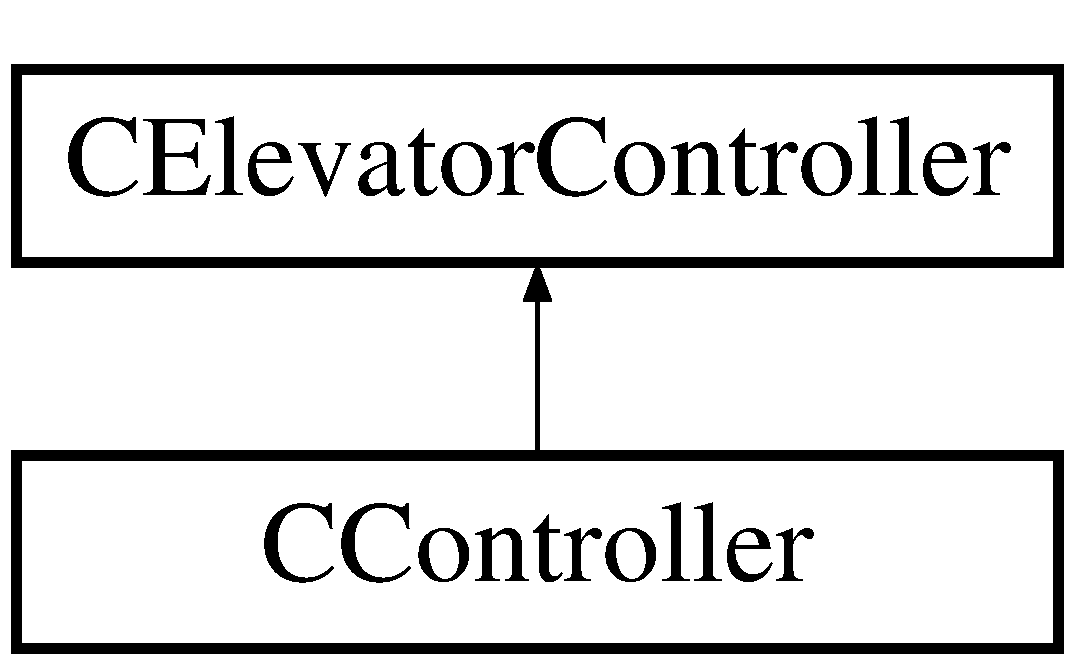
\includegraphics[height=2.000000cm]{class_c_controller}
\end{center}
\end{figure}
\subsection*{Public Types}
\begin{DoxyCompactItemize}
\item 
\hypertarget{class_c_controller_a4c332e7b3c3035cdde7b8f344b565429}{enum \hyperlink{class_c_controller_a4c332e7b3c3035cdde7b8f344b565429}{States} \{ \\*
{\bfseries Idle}, 
{\bfseries Door\+Opening}, 
{\bfseries Door\+Open}, 
{\bfseries Door\+Closing}, 
\\*
{\bfseries Moving}, 
{\bfseries Stop}, 
{\bfseries Fireman\+Mode\+Idle}, 
{\bfseries Fireman\+Mode\+Opening}, 
\\*
{\bfseries Fireman\+Mode\+Closing}, 
{\bfseries Fireman\+Mode\+Moving}, 
{\bfseries Fireman\+Mode\+Stop}, 
{\bfseries Fireman\+Mode\+Closed}
 \}}\label{class_c_controller_a4c332e7b3c3035cdde7b8f344b565429}

\begin{DoxyCompactList}\small\item\em The state machine states. \end{DoxyCompactList}\end{DoxyCompactItemize}
\subsection*{Public Member Functions}
\begin{DoxyCompactItemize}
\item 
\hypertarget{class_c_controller_a840d9cb376c21b58566c7f9c069e402f}{\hyperlink{class_c_controller_a840d9cb376c21b58566c7f9c069e402f}{C\+Controller} ()}\label{class_c_controller_a840d9cb376c21b58566c7f9c069e402f}

\begin{DoxyCompactList}\small\item\em Constructor. \end{DoxyCompactList}\item 
\hypertarget{class_c_controller_a06c1bf4eeb697d4f7574ea1d7c51d267}{virtual \hyperlink{class_c_controller_a06c1bf4eeb697d4f7574ea1d7c51d267}{$\sim$\+C\+Controller} ()}\label{class_c_controller_a06c1bf4eeb697d4f7574ea1d7c51d267}

\begin{DoxyCompactList}\small\item\em Virtual Destructor. \end{DoxyCompactList}\item 
virtual void \hyperlink{class_c_controller_a6d6c0e9fc0c9d8dac6c16d6c077f0863}{Service} () override
\begin{DoxyCompactList}\small\item\em Elevator service function. \end{DoxyCompactList}\item 
\hypertarget{class_c_controller_a6be672a805c6643891a54711cce3e64d}{void \hyperlink{class_c_controller_a6be672a805c6643891a54711cce3e64d}{Initialize} ()}\label{class_c_controller_a6be672a805c6643891a54711cce3e64d}

\begin{DoxyCompactList}\small\item\em Initializes the controller. \end{DoxyCompactList}\item 
virtual void \hyperlink{class_c_controller_ac0f1d0ba9728974024a921cd2e372fc2}{On\+Open\+Pressed} () override
\begin{DoxyCompactList}\small\item\em This function is called when the open button is pressed. \end{DoxyCompactList}\item 
\hypertarget{class_c_controller_a4572ee70739d93ebf98db14ee85812b1}{virtual void \hyperlink{class_c_controller_a4572ee70739d93ebf98db14ee85812b1}{On\+Close\+Pressed} () override}\label{class_c_controller_a4572ee70739d93ebf98db14ee85812b1}

\begin{DoxyCompactList}\small\item\em This function is called when the door close button is pressed. \end{DoxyCompactList}\item 
virtual void \hyperlink{class_c_controller_a51a8022c7acbf95ffa907ff063899713}{On\+Panel\+Floor\+Pressed} (int floor) override
\begin{DoxyCompactList}\small\item\em Function is called when the panel floor is pressed. \end{DoxyCompactList}\item 
virtual void \hyperlink{class_c_controller_af00ba0b3ea16235cd1f0e6f1fe672526}{On\+Call\+Up\+Pressed} (int floor) override
\begin{DoxyCompactList}\small\item\em Function called when the call-\/up elevator button is pressed. \end{DoxyCompactList}\item 
virtual void \hyperlink{class_c_controller_ac542dad16cba63af452184e3878e8d8e}{On\+Call\+Down\+Pressed} (int floor) override
\begin{DoxyCompactList}\small\item\em Function called when the call-\/down elevator button is pressed. \end{DoxyCompactList}\end{DoxyCompactItemize}


\subsection{Detailed Description}
An extended elevator controller class. 

\subsection{Member Function Documentation}
\hypertarget{class_c_controller_ac542dad16cba63af452184e3878e8d8e}{\index{C\+Controller@{C\+Controller}!On\+Call\+Down\+Pressed@{On\+Call\+Down\+Pressed}}
\index{On\+Call\+Down\+Pressed@{On\+Call\+Down\+Pressed}!C\+Controller@{C\+Controller}}
\subsubsection[{On\+Call\+Down\+Pressed}]{\setlength{\rightskip}{0pt plus 5cm}void C\+Controller\+::\+On\+Call\+Down\+Pressed (
\begin{DoxyParamCaption}
\item[{int}]{floor}
\end{DoxyParamCaption}
)\hspace{0.3cm}{\ttfamily [override]}, {\ttfamily [virtual]}}}\label{class_c_controller_ac542dad16cba63af452184e3878e8d8e}


Function called when the call-\/down elevator button is pressed. 


\begin{DoxyParams}{Parameters}
{\em floor} & -\/ The floor called on (int) \\
\hline
\end{DoxyParams}
\hypertarget{class_c_controller_af00ba0b3ea16235cd1f0e6f1fe672526}{\index{C\+Controller@{C\+Controller}!On\+Call\+Up\+Pressed@{On\+Call\+Up\+Pressed}}
\index{On\+Call\+Up\+Pressed@{On\+Call\+Up\+Pressed}!C\+Controller@{C\+Controller}}
\subsubsection[{On\+Call\+Up\+Pressed}]{\setlength{\rightskip}{0pt plus 5cm}void C\+Controller\+::\+On\+Call\+Up\+Pressed (
\begin{DoxyParamCaption}
\item[{int}]{floor}
\end{DoxyParamCaption}
)\hspace{0.3cm}{\ttfamily [override]}, {\ttfamily [virtual]}}}\label{class_c_controller_af00ba0b3ea16235cd1f0e6f1fe672526}


Function called when the call-\/up elevator button is pressed. 


\begin{DoxyParams}{Parameters}
{\em floor} & -\/ The int of the floor \\
\hline
\end{DoxyParams}
\hypertarget{class_c_controller_ac0f1d0ba9728974024a921cd2e372fc2}{\index{C\+Controller@{C\+Controller}!On\+Open\+Pressed@{On\+Open\+Pressed}}
\index{On\+Open\+Pressed@{On\+Open\+Pressed}!C\+Controller@{C\+Controller}}
\subsubsection[{On\+Open\+Pressed}]{\setlength{\rightskip}{0pt plus 5cm}void C\+Controller\+::\+On\+Open\+Pressed (
\begin{DoxyParamCaption}
{}
\end{DoxyParamCaption}
)\hspace{0.3cm}{\ttfamily [override]}, {\ttfamily [virtual]}}}\label{class_c_controller_ac0f1d0ba9728974024a921cd2e372fc2}


This function is called when the open button is pressed. 

Event Handlers \hypertarget{class_c_controller_a51a8022c7acbf95ffa907ff063899713}{\index{C\+Controller@{C\+Controller}!On\+Panel\+Floor\+Pressed@{On\+Panel\+Floor\+Pressed}}
\index{On\+Panel\+Floor\+Pressed@{On\+Panel\+Floor\+Pressed}!C\+Controller@{C\+Controller}}
\subsubsection[{On\+Panel\+Floor\+Pressed}]{\setlength{\rightskip}{0pt plus 5cm}void C\+Controller\+::\+On\+Panel\+Floor\+Pressed (
\begin{DoxyParamCaption}
\item[{int}]{floor}
\end{DoxyParamCaption}
)\hspace{0.3cm}{\ttfamily [override]}, {\ttfamily [virtual]}}}\label{class_c_controller_a51a8022c7acbf95ffa907ff063899713}


Function is called when the panel floor is pressed. 


\begin{DoxyParams}{Parameters}
{\em floor} & -\/ The int of the floor it was pressed on \\
\hline
\end{DoxyParams}
\hypertarget{class_c_controller_a6d6c0e9fc0c9d8dac6c16d6c077f0863}{\index{C\+Controller@{C\+Controller}!Service@{Service}}
\index{Service@{Service}!C\+Controller@{C\+Controller}}
\subsubsection[{Service}]{\setlength{\rightskip}{0pt plus 5cm}void C\+Controller\+::\+Service (
\begin{DoxyParamCaption}
{}
\end{DoxyParamCaption}
)\hspace{0.3cm}{\ttfamily [override]}, {\ttfamily [virtual]}}}\label{class_c_controller_a6d6c0e9fc0c9d8dac6c16d6c077f0863}


Elevator service function. 

General Functions\+This function is called once every 0.\+001 seconds and allows us to control elevator functionality.

This function is called once every 0.\+001 seconds and allows us to control elevator functionality. Fireman Mode 

The documentation for this class was generated from the following files\+:\begin{DoxyCompactItemize}
\item 
\hyperlink{_controller_8h}{Controller.\+h}\item 
\hyperlink{_controller_8cpp}{Controller.\+cpp}\end{DoxyCompactItemize}

\hypertarget{class_c_floor}{\section{C\+Floor Class Reference}
\label{class_c_floor}\index{C\+Floor@{C\+Floor}}
}


Represents a floor.  




{\ttfamily \#include $<$Floor.\+h$>$}

\subsection*{Public Member Functions}
\begin{DoxyCompactItemize}
\item 
\hypertarget{class_c_floor_af437bdb8f830e3ecf6f19d6eebdf56c1}{\hyperlink{class_c_floor_af437bdb8f830e3ecf6f19d6eebdf56c1}{C\+Floor} ()}\label{class_c_floor_af437bdb8f830e3ecf6f19d6eebdf56c1}

\begin{DoxyCompactList}\small\item\em Cosntructor. \end{DoxyCompactList}\item 
\hypertarget{class_c_floor_abd1acd7879d4eb83db8792db677ace93}{virtual \hyperlink{class_c_floor_abd1acd7879d4eb83db8792db677ace93}{$\sim$\+C\+Floor} ()}\label{class_c_floor_abd1acd7879d4eb83db8792db677ace93}

\begin{DoxyCompactList}\small\item\em Destructor. \end{DoxyCompactList}\item 
bool \hyperlink{class_c_floor_a2d23e56c8799fe99e18436f71aad84e5}{Is\+Up} ()
\begin{DoxyCompactList}\small\item\em Gets the up flag (true if moving up) \end{DoxyCompactList}\item 
void \hyperlink{class_c_floor_a130545e2b7d76da50bf6413fc704cfa7}{Set\+Up} (bool flag)
\begin{DoxyCompactList}\small\item\em Sets the up flag (true if moving up) \end{DoxyCompactList}\item 
bool \hyperlink{class_c_floor_aef3cf57dbac94449f936517715fbfe38}{Is\+Down} ()
\begin{DoxyCompactList}\small\item\em Gets the down flag (true if moving down) \end{DoxyCompactList}\item 
void \hyperlink{class_c_floor_aa9c11f1b254e2036169c64738a1b1ba4}{Set\+Down} (bool flag)
\begin{DoxyCompactList}\small\item\em Sets the down flag (true if moving down) \end{DoxyCompactList}\item 
bool \hyperlink{class_c_floor_abe6e792f63d6bd19ab7736acbb62d3db}{Is\+Panel} ()
\begin{DoxyCompactList}\small\item\em Gets the panel flag (...) \end{DoxyCompactList}\item 
void \hyperlink{class_c_floor_a3eb3317a74f098cd7a177d097ca84f86}{Set\+Panel} (bool flag)
\begin{DoxyCompactList}\small\item\em Sets the panel flag (...) \end{DoxyCompactList}\item 
int \hyperlink{class_c_floor_abff3a5ae38b20daaef8acffe46bc5b29}{Get\+Floor} ()
\begin{DoxyCompactList}\small\item\em Gets the floor number. \end{DoxyCompactList}\item 
void \hyperlink{class_c_floor_a8bea33b2504b95f1e50c0590e166c93a}{Set\+Floor} (int floor)
\begin{DoxyCompactList}\small\item\em Sets the floor number. \end{DoxyCompactList}\item 
\hyperlink{class_c_controller}{C\+Controller} $\ast$ \hyperlink{class_c_floor_a917d1bd7d2dbb16fd3eb5719cde350ee}{Get\+Controller} ()
\begin{DoxyCompactList}\small\item\em Gets the controller object. \end{DoxyCompactList}\item 
void \hyperlink{class_c_floor_a341290d360881779fdf30198e4d37f54}{Set\+Controller} (\hyperlink{class_c_controller}{C\+Controller} $\ast$controller)
\begin{DoxyCompactList}\small\item\em Sets the controller object. \end{DoxyCompactList}\end{DoxyCompactItemize}


\subsection{Detailed Description}
Represents a floor. 

\subsection{Member Function Documentation}
\hypertarget{class_c_floor_a917d1bd7d2dbb16fd3eb5719cde350ee}{\index{C\+Floor@{C\+Floor}!Get\+Controller@{Get\+Controller}}
\index{Get\+Controller@{Get\+Controller}!C\+Floor@{C\+Floor}}
\subsubsection[{Get\+Controller}]{\setlength{\rightskip}{0pt plus 5cm}{\bf C\+Controller}$\ast$ C\+Floor\+::\+Get\+Controller (
\begin{DoxyParamCaption}
{}
\end{DoxyParamCaption}
)\hspace{0.3cm}{\ttfamily [inline]}}}\label{class_c_floor_a917d1bd7d2dbb16fd3eb5719cde350ee}


Gets the controller object. 

\begin{DoxyReturn}{Returns}
a pointer to the controller 
\end{DoxyReturn}
\hypertarget{class_c_floor_abff3a5ae38b20daaef8acffe46bc5b29}{\index{C\+Floor@{C\+Floor}!Get\+Floor@{Get\+Floor}}
\index{Get\+Floor@{Get\+Floor}!C\+Floor@{C\+Floor}}
\subsubsection[{Get\+Floor}]{\setlength{\rightskip}{0pt plus 5cm}int C\+Floor\+::\+Get\+Floor (
\begin{DoxyParamCaption}
{}
\end{DoxyParamCaption}
)\hspace{0.3cm}{\ttfamily [inline]}}}\label{class_c_floor_abff3a5ae38b20daaef8acffe46bc5b29}


Gets the floor number. 

\begin{DoxyReturn}{Returns}
int representing the floor 
\end{DoxyReturn}
\hypertarget{class_c_floor_aef3cf57dbac94449f936517715fbfe38}{\index{C\+Floor@{C\+Floor}!Is\+Down@{Is\+Down}}
\index{Is\+Down@{Is\+Down}!C\+Floor@{C\+Floor}}
\subsubsection[{Is\+Down}]{\setlength{\rightskip}{0pt plus 5cm}bool C\+Floor\+::\+Is\+Down (
\begin{DoxyParamCaption}
{}
\end{DoxyParamCaption}
)\hspace{0.3cm}{\ttfamily [inline]}}}\label{class_c_floor_aef3cf57dbac94449f936517715fbfe38}


Gets the down flag (true if moving down) 

\begin{DoxyReturn}{Returns}
true if we are going down 
\end{DoxyReturn}
\hypertarget{class_c_floor_abe6e792f63d6bd19ab7736acbb62d3db}{\index{C\+Floor@{C\+Floor}!Is\+Panel@{Is\+Panel}}
\index{Is\+Panel@{Is\+Panel}!C\+Floor@{C\+Floor}}
\subsubsection[{Is\+Panel}]{\setlength{\rightskip}{0pt plus 5cm}bool C\+Floor\+::\+Is\+Panel (
\begin{DoxyParamCaption}
{}
\end{DoxyParamCaption}
)\hspace{0.3cm}{\ttfamily [inline]}}}\label{class_c_floor_abe6e792f63d6bd19ab7736acbb62d3db}


Gets the panel flag (...) 

\begin{DoxyReturn}{Returns}
true if we are a panel 
\end{DoxyReturn}
\hypertarget{class_c_floor_a2d23e56c8799fe99e18436f71aad84e5}{\index{C\+Floor@{C\+Floor}!Is\+Up@{Is\+Up}}
\index{Is\+Up@{Is\+Up}!C\+Floor@{C\+Floor}}
\subsubsection[{Is\+Up}]{\setlength{\rightskip}{0pt plus 5cm}bool C\+Floor\+::\+Is\+Up (
\begin{DoxyParamCaption}
{}
\end{DoxyParamCaption}
)\hspace{0.3cm}{\ttfamily [inline]}}}\label{class_c_floor_a2d23e56c8799fe99e18436f71aad84e5}


Gets the up flag (true if moving up) 

Getters \& Setters\begin{DoxyReturn}{Returns}
true if we are going up 
\end{DoxyReturn}
\hypertarget{class_c_floor_a341290d360881779fdf30198e4d37f54}{\index{C\+Floor@{C\+Floor}!Set\+Controller@{Set\+Controller}}
\index{Set\+Controller@{Set\+Controller}!C\+Floor@{C\+Floor}}
\subsubsection[{Set\+Controller}]{\setlength{\rightskip}{0pt plus 5cm}void C\+Floor\+::\+Set\+Controller (
\begin{DoxyParamCaption}
\item[{{\bf C\+Controller} $\ast$}]{controller}
\end{DoxyParamCaption}
)\hspace{0.3cm}{\ttfamily [inline]}}}\label{class_c_floor_a341290d360881779fdf30198e4d37f54}


Sets the controller object. 


\begin{DoxyParams}{Parameters}
{\em controller} & -\/ the controller this guy belongs to \\
\hline
\end{DoxyParams}
\hypertarget{class_c_floor_aa9c11f1b254e2036169c64738a1b1ba4}{\index{C\+Floor@{C\+Floor}!Set\+Down@{Set\+Down}}
\index{Set\+Down@{Set\+Down}!C\+Floor@{C\+Floor}}
\subsubsection[{Set\+Down}]{\setlength{\rightskip}{0pt plus 5cm}void C\+Floor\+::\+Set\+Down (
\begin{DoxyParamCaption}
\item[{bool}]{flag}
\end{DoxyParamCaption}
)}}\label{class_c_floor_aa9c11f1b254e2036169c64738a1b1ba4}


Sets the down flag (true if moving down) 

Set the value of Panel for a floor.


\begin{DoxyParams}{Parameters}
{\em flag} & -\/ The flag to set to\\
\hline
{\em flag} & -\/ The new value for m\+Panel \\
\hline
\end{DoxyParams}
\hypertarget{class_c_floor_a8bea33b2504b95f1e50c0590e166c93a}{\index{C\+Floor@{C\+Floor}!Set\+Floor@{Set\+Floor}}
\index{Set\+Floor@{Set\+Floor}!C\+Floor@{C\+Floor}}
\subsubsection[{Set\+Floor}]{\setlength{\rightskip}{0pt plus 5cm}void C\+Floor\+::\+Set\+Floor (
\begin{DoxyParamCaption}
\item[{int}]{floor}
\end{DoxyParamCaption}
)\hspace{0.3cm}{\ttfamily [inline]}}}\label{class_c_floor_a8bea33b2504b95f1e50c0590e166c93a}


Sets the floor number. 


\begin{DoxyParams}{Parameters}
{\em floor} & -\/ The floor number to set to \\
\hline
\end{DoxyParams}
\hypertarget{class_c_floor_a3eb3317a74f098cd7a177d097ca84f86}{\index{C\+Floor@{C\+Floor}!Set\+Panel@{Set\+Panel}}
\index{Set\+Panel@{Set\+Panel}!C\+Floor@{C\+Floor}}
\subsubsection[{Set\+Panel}]{\setlength{\rightskip}{0pt plus 5cm}void C\+Floor\+::\+Set\+Panel (
\begin{DoxyParamCaption}
\item[{bool}]{flag}
\end{DoxyParamCaption}
)}}\label{class_c_floor_a3eb3317a74f098cd7a177d097ca84f86}


Sets the panel flag (...) 

Set the value of Panel for a floor.


\begin{DoxyParams}{Parameters}
{\em flag} & -\/ The flag to set to\\
\hline
{\em flag} & The new value for m\+Panel \\
\hline
\end{DoxyParams}
\hypertarget{class_c_floor_a130545e2b7d76da50bf6413fc704cfa7}{\index{C\+Floor@{C\+Floor}!Set\+Up@{Set\+Up}}
\index{Set\+Up@{Set\+Up}!C\+Floor@{C\+Floor}}
\subsubsection[{Set\+Up}]{\setlength{\rightskip}{0pt plus 5cm}void C\+Floor\+::\+Set\+Up (
\begin{DoxyParamCaption}
\item[{bool}]{flag}
\end{DoxyParamCaption}
)}}\label{class_c_floor_a130545e2b7d76da50bf6413fc704cfa7}


Sets the up flag (true if moving up) 


\begin{DoxyParams}{Parameters}
{\em flag} & -\/ The flag to set to \\
\hline
\end{DoxyParams}


The documentation for this class was generated from the following files\+:\begin{DoxyCompactItemize}
\item 
\hyperlink{_floor_8h}{Floor.\+h}\item 
\hyperlink{_floor_8cpp}{Floor.\+cpp}\end{DoxyCompactItemize}

\hypertarget{class_c_main_frame}{\section{C\+Main\+Frame Class Reference}
\label{class_c_main_frame}\index{C\+Main\+Frame@{C\+Main\+Frame}}
}


Program main frame.  




{\ttfamily \#include $<$Main\+Frm.\+h$>$}

Inheritance diagram for C\+Main\+Frame\+:\begin{figure}[H]
\begin{center}
\leavevmode
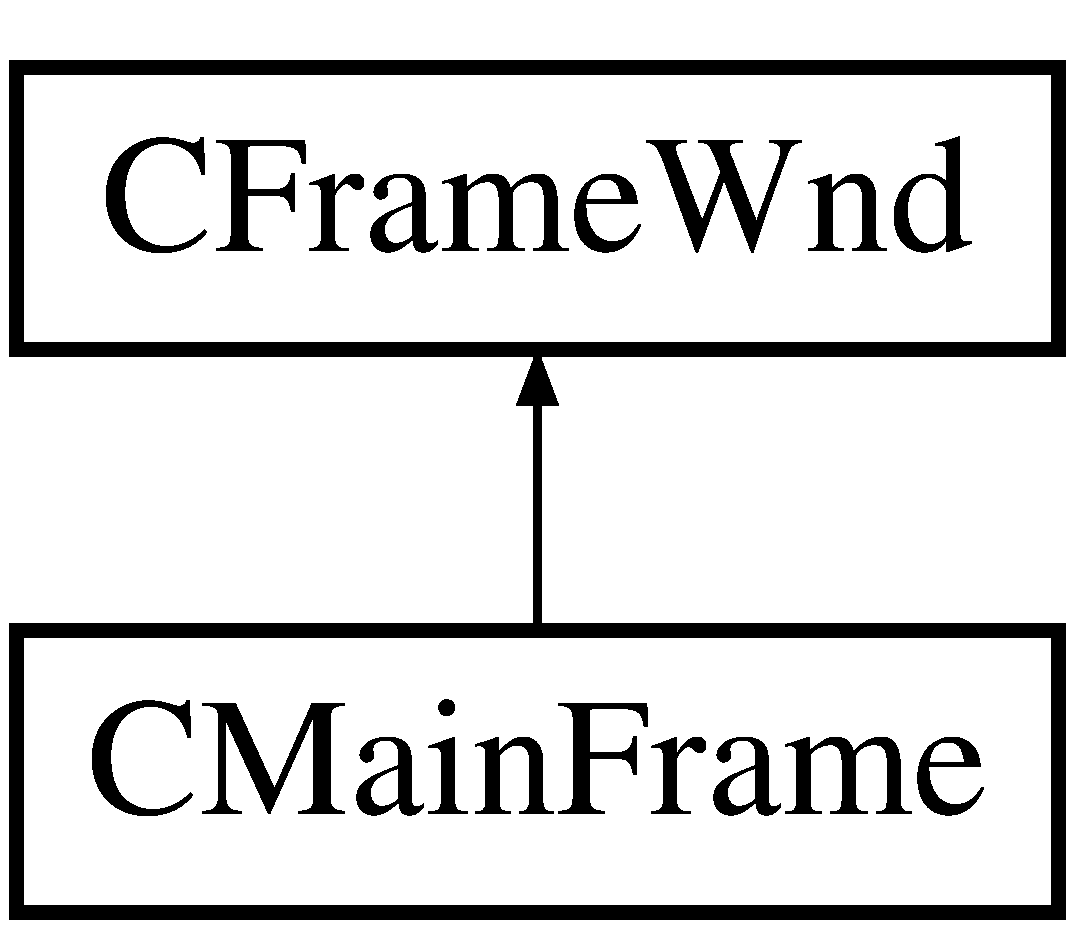
\includegraphics[height=2.000000cm]{class_c_main_frame}
\end{center}
\end{figure}
\subsection*{Public Types}
\begin{DoxyCompactItemize}
\item 
\hypertarget{class_c_main_frame_a89722c82d82f95a761772a8dd9755b7b}{enum \hyperlink{class_c_main_frame_a89722c82d82f95a761772a8dd9755b7b}{Motion\+Modes} \{ {\bfseries Move}, 
{\bfseries Rotate}
 \}}\label{class_c_main_frame_a89722c82d82f95a761772a8dd9755b7b}

\begin{DoxyCompactList}\small\item\em Enumerations for the possible manipulation modes. \end{DoxyCompactList}\end{DoxyCompactItemize}
\subsection*{Public Member Functions}
\begin{DoxyCompactItemize}
\item 
\hypertarget{class_c_main_frame_af3e997aeae4148d2aaa4a1e1ae7bdd53}{\hyperlink{class_c_main_frame_af3e997aeae4148d2aaa4a1e1ae7bdd53}{C\+Main\+Frame} ()}\label{class_c_main_frame_af3e997aeae4148d2aaa4a1e1ae7bdd53}

\begin{DoxyCompactList}\small\item\em Constructor. \end{DoxyCompactList}\item 
\hyperlink{class_c_main_frame_a89722c82d82f95a761772a8dd9755b7b}{Motion\+Modes} \hyperlink{class_c_main_frame_a76c571ab75752dba8049e08f5e4ac920}{Get\+Mode} () const 
\begin{DoxyCompactList}\small\item\em The selected manipulation mode. \end{DoxyCompactList}\item 
\hypertarget{class_c_main_frame_a549bf677c955c2898c3c683321633c16}{virtual B\+O\+O\+L {\bfseries Pre\+Create\+Window} (C\+R\+E\+A\+T\+E\+S\+T\+R\+U\+C\+T \&cs)}\label{class_c_main_frame_a549bf677c955c2898c3c683321633c16}

\item 
\hypertarget{class_c_main_frame_ade959eb0bab719bf06bb9b18ee407101}{virtual B\+O\+O\+L {\bfseries On\+Cmd\+Msg} (U\+I\+N\+T n\+I\+D, int n\+Code, void $\ast$p\+Extra, A\+F\+X\+\_\+\+C\+M\+D\+H\+A\+N\+D\+L\+E\+R\+I\+N\+F\+O $\ast$p\+Handler\+Info)}\label{class_c_main_frame_ade959eb0bab719bf06bb9b18ee407101}

\item 
\hypertarget{class_c_main_frame_a8ae555f23fdf97edb4feb4d3e1bfa4ee}{virtual \hyperlink{class_c_main_frame_a8ae555f23fdf97edb4feb4d3e1bfa4ee}{$\sim$\+C\+Main\+Frame} ()}\label{class_c_main_frame_a8ae555f23fdf97edb4feb4d3e1bfa4ee}

\begin{DoxyCompactList}\small\item\em Destructor. \end{DoxyCompactList}\item 
afx\+\_\+msg void \hyperlink{class_c_main_frame_adf171bf1f2c6f10cc85dbe8db3fc93f7}{On\+Size} (U\+I\+N\+T n\+Type, int cx, int cy)
\begin{DoxyCompactList}\small\item\em Handle a Size request from Windows. \end{DoxyCompactList}\item 
afx\+\_\+msg B\+O\+O\+L \hyperlink{class_c_main_frame_a53a97f2229c5765329b2b59a21a54b0d}{On\+Erase\+Bkgnd} (C\+D\+C $\ast$p\+D\+C)
\begin{DoxyCompactList}\small\item\em Called to erase the background. Disabled so we don't get flicker. \end{DoxyCompactList}\item 
\hypertarget{class_c_main_frame_af07c2610f9f5631e7eb7374d10d5fdd3}{afx\+\_\+msg void \hyperlink{class_c_main_frame_af07c2610f9f5631e7eb7374d10d5fdd3}{On\+Edit\+Move} ()}\label{class_c_main_frame_af07c2610f9f5631e7eb7374d10d5fdd3}

\begin{DoxyCompactList}\small\item\em Handle the Edit$>$Mode menu option. \end{DoxyCompactList}\item 
afx\+\_\+msg void \hyperlink{class_c_main_frame_aadc40c4ab290da2368f6b87443f5ffbc}{On\+Update\+Edit\+Move} (C\+Cmd\+U\+I $\ast$p\+Cmd\+U\+I)
\begin{DoxyCompactList}\small\item\em Update the menu for Edit$>$Move. \end{DoxyCompactList}\item 
\hypertarget{class_c_main_frame_a00f10667f35de1fa6693c1bea941d878}{afx\+\_\+msg void \hyperlink{class_c_main_frame_a00f10667f35de1fa6693c1bea941d878}{On\+Edit\+Rotate} ()}\label{class_c_main_frame_a00f10667f35de1fa6693c1bea941d878}

\begin{DoxyCompactList}\small\item\em Handle the Edit$>$Rotate menu option. \end{DoxyCompactList}\item 
afx\+\_\+msg void \hyperlink{class_c_main_frame_af098b8129775d1b5fb47fcaaabce8c01}{On\+Update\+Edit\+Rotate} (C\+Cmd\+U\+I $\ast$p\+Cmd\+U\+I)
\begin{DoxyCompactList}\small\item\em Update the menu for Edit$>$Rotate. \end{DoxyCompactList}\end{DoxyCompactItemize}
\subsection*{Protected Member Functions}
\begin{DoxyCompactItemize}
\item 
\hypertarget{class_c_main_frame_a48666466fd37412fcaeff75c3b12e0ed}{afx\+\_\+msg int {\bfseries On\+Create} (L\+P\+C\+R\+E\+A\+T\+E\+S\+T\+R\+U\+C\+T lp\+Create\+Struct)}\label{class_c_main_frame_a48666466fd37412fcaeff75c3b12e0ed}

\item 
\hypertarget{class_c_main_frame_adc353a3d1fc497fbc009b6d9e6914a82}{afx\+\_\+msg void {\bfseries On\+Set\+Focus} (C\+Wnd $\ast$p\+Old\+Wnd)}\label{class_c_main_frame_adc353a3d1fc497fbc009b6d9e6914a82}

\item 
\hypertarget{class_c_main_frame_ac863d694fd3637d492ef97396defbd8e}{virtual B\+O\+O\+L {\bfseries On\+Create\+Client} (L\+P\+C\+R\+E\+A\+T\+E\+S\+T\+R\+U\+C\+T lpcs, C\+Create\+Context $\ast$p\+Context)}\label{class_c_main_frame_ac863d694fd3637d492ef97396defbd8e}

\end{DoxyCompactItemize}
\subsection*{Protected Attributes}
\begin{DoxyCompactItemize}
\item 
\hypertarget{class_c_main_frame_ac8558942627d1502b5095e736840a1f3}{C\+M\+F\+C\+Tool\+Bar {\bfseries m\+\_\+wnd\+Tool\+Bar}}\label{class_c_main_frame_ac8558942627d1502b5095e736840a1f3}

\item 
\hypertarget{class_c_main_frame_a5842bded00e9137fbbf77343b99863be}{C\+M\+F\+C\+Status\+Bar {\bfseries m\+\_\+wnd\+Status\+Bar}}\label{class_c_main_frame_a5842bded00e9137fbbf77343b99863be}

\item 
\hypertarget{class_c_main_frame_a1d68466db594c4bebf41f707bc0a0647}{C\+Splitter\+Wnd {\bfseries m\+Wnd\+Splitter}}\label{class_c_main_frame_a1d68466db594c4bebf41f707bc0a0647}

\end{DoxyCompactItemize}


\subsection{Detailed Description}
Program main frame. 

\subsection{Member Function Documentation}
\hypertarget{class_c_main_frame_a76c571ab75752dba8049e08f5e4ac920}{\index{C\+Main\+Frame@{C\+Main\+Frame}!Get\+Mode@{Get\+Mode}}
\index{Get\+Mode@{Get\+Mode}!C\+Main\+Frame@{C\+Main\+Frame}}
\subsubsection[{Get\+Mode}]{\setlength{\rightskip}{0pt plus 5cm}{\bf Motion\+Modes} C\+Main\+Frame\+::\+Get\+Mode (
\begin{DoxyParamCaption}
{}
\end{DoxyParamCaption}
) const\hspace{0.3cm}{\ttfamily [inline]}}}\label{class_c_main_frame_a76c571ab75752dba8049e08f5e4ac920}


The selected manipulation mode. 

\begin{DoxyReturn}{Returns}
Currently selected manipulation mode 
\end{DoxyReturn}
\hypertarget{class_c_main_frame_a53a97f2229c5765329b2b59a21a54b0d}{\index{C\+Main\+Frame@{C\+Main\+Frame}!On\+Erase\+Bkgnd@{On\+Erase\+Bkgnd}}
\index{On\+Erase\+Bkgnd@{On\+Erase\+Bkgnd}!C\+Main\+Frame@{C\+Main\+Frame}}
\subsubsection[{On\+Erase\+Bkgnd}]{\setlength{\rightskip}{0pt plus 5cm}B\+O\+O\+L C\+Main\+Frame\+::\+On\+Erase\+Bkgnd (
\begin{DoxyParamCaption}
\item[{C\+D\+C $\ast$}]{p\+D\+C}
\end{DoxyParamCaption}
)}}\label{class_c_main_frame_a53a97f2229c5765329b2b59a21a54b0d}


Called to erase the background. Disabled so we don't get flicker. 


\begin{DoxyParams}{Parameters}
{\em p\+D\+C} & A device context \\
\hline
\end{DoxyParams}
\begin{DoxyReturn}{Returns}
F\+A\+L\+S\+E 
\end{DoxyReturn}
\hypertarget{class_c_main_frame_adf171bf1f2c6f10cc85dbe8db3fc93f7}{\index{C\+Main\+Frame@{C\+Main\+Frame}!On\+Size@{On\+Size}}
\index{On\+Size@{On\+Size}!C\+Main\+Frame@{C\+Main\+Frame}}
\subsubsection[{On\+Size}]{\setlength{\rightskip}{0pt plus 5cm}void C\+Main\+Frame\+::\+On\+Size (
\begin{DoxyParamCaption}
\item[{U\+I\+N\+T}]{n\+Type, }
\item[{int}]{cx, }
\item[{int}]{cy}
\end{DoxyParamCaption}
)}}\label{class_c_main_frame_adf171bf1f2c6f10cc85dbe8db3fc93f7}


Handle a Size request from Windows. 

This function ensures the child windows are the correct size on the screen after the main window is resized 
\begin{DoxyParams}{Parameters}
{\em n\+Type} & Type of resizing message \\
\hline
{\em cx} & The new width \\
\hline
{\em cy} & The new height \\
\hline
\end{DoxyParams}
\hypertarget{class_c_main_frame_aadc40c4ab290da2368f6b87443f5ffbc}{\index{C\+Main\+Frame@{C\+Main\+Frame}!On\+Update\+Edit\+Move@{On\+Update\+Edit\+Move}}
\index{On\+Update\+Edit\+Move@{On\+Update\+Edit\+Move}!C\+Main\+Frame@{C\+Main\+Frame}}
\subsubsection[{On\+Update\+Edit\+Move}]{\setlength{\rightskip}{0pt plus 5cm}void C\+Main\+Frame\+::\+On\+Update\+Edit\+Move (
\begin{DoxyParamCaption}
\item[{C\+Cmd\+U\+I $\ast$}]{p\+Cmd\+U\+I}
\end{DoxyParamCaption}
)}}\label{class_c_main_frame_aadc40c4ab290da2368f6b87443f5ffbc}


Update the menu for Edit$>$Move. 


\begin{DoxyParams}{Parameters}
{\em p\+Cmd\+U\+I} & The pointer to the control user interface \\
\hline
\end{DoxyParams}
\hypertarget{class_c_main_frame_af098b8129775d1b5fb47fcaaabce8c01}{\index{C\+Main\+Frame@{C\+Main\+Frame}!On\+Update\+Edit\+Rotate@{On\+Update\+Edit\+Rotate}}
\index{On\+Update\+Edit\+Rotate@{On\+Update\+Edit\+Rotate}!C\+Main\+Frame@{C\+Main\+Frame}}
\subsubsection[{On\+Update\+Edit\+Rotate}]{\setlength{\rightskip}{0pt plus 5cm}void C\+Main\+Frame\+::\+On\+Update\+Edit\+Rotate (
\begin{DoxyParamCaption}
\item[{C\+Cmd\+U\+I $\ast$}]{p\+Cmd\+U\+I}
\end{DoxyParamCaption}
)}}\label{class_c_main_frame_af098b8129775d1b5fb47fcaaabce8c01}


Update the menu for Edit$>$Rotate. 


\begin{DoxyParams}{Parameters}
{\em p\+Cmd\+U\+I} & The pointer to the control user interface \\
\hline
\end{DoxyParams}


The documentation for this class was generated from the following files\+:\begin{DoxyCompactItemize}
\item 
\hyperlink{_main_frm_8h}{Main\+Frm.\+h}\item 
\hyperlink{_main_frm_8cpp}{Main\+Frm.\+cpp}\end{DoxyCompactItemize}

\chapter{File Documentation}
\hypertarget{_controller_8cpp}{\section{Controller.\+cpp File Reference}
\label{_controller_8cpp}\index{Controller.\+cpp@{Controller.\+cpp}}
}
{\ttfamily \#include \char`\"{}stdafx.\+h\char`\"{}}\\*
{\ttfamily \#include \char`\"{}Controller.\+h\char`\"{}}\\*
\subsection*{Variables}
\begin{DoxyCompactItemize}
\item 
\hypertarget{_controller_8cpp_a53f694a39b59d40e3f585ced7bbe514b}{const double \hyperlink{_controller_8cpp_a53f694a39b59d40e3f585ced7bbe514b}{Door\+Open\+Time} = 2.\+0}\label{_controller_8cpp_a53f694a39b59d40e3f585ced7bbe514b}

\begin{DoxyCompactList}\small\item\em The time the door remains open. \end{DoxyCompactList}\item 
\hypertarget{_controller_8cpp_a1a532391f6564bf78e699715f21161bc}{const double \hyperlink{_controller_8cpp_a1a532391f6564bf78e699715f21161bc}{Stop\+Open\+Time} = 1.\+0}\label{_controller_8cpp_a1a532391f6564bf78e699715f21161bc}

\begin{DoxyCompactList}\small\item\em The time till the doors open once it stops at a floor. \end{DoxyCompactList}\item 
\hypertarget{_controller_8cpp_a7bd0aadacd0c450bce0da97665241930}{const int \hyperlink{_controller_8cpp_a7bd0aadacd0c450bce0da97665241930}{Fireman\+Floor} = 1}\label{_controller_8cpp_a7bd0aadacd0c450bce0da97665241930}

\begin{DoxyCompactList}\small\item\em The floor to go to in fireman mode. \end{DoxyCompactList}\end{DoxyCompactItemize}


\subsection{Detailed Description}
\begin{DoxyAuthor}{Author}
Charles Bean 
\end{DoxyAuthor}

\hypertarget{_controller_8h}{\section{Controller.\+h File Reference}
\label{_controller_8h}\index{Controller.\+h@{Controller.\+h}}
}


The controller for our elevator library -\/ it extends the libraries controller.  


{\ttfamily \#include \char`\"{}Elevator\+Controller.\+h\char`\"{}}\\*
{\ttfamily \#include \char`\"{}Floor.\+h\char`\"{}}\\*
\subsection*{Classes}
\begin{DoxyCompactItemize}
\item 
class \hyperlink{class_c_controller}{C\+Controller}
\begin{DoxyCompactList}\small\item\em An extended elevator controller class. \end{DoxyCompactList}\end{DoxyCompactItemize}


\subsection{Detailed Description}
The controller for our elevator library -\/ it extends the libraries controller. 

\begin{DoxyAuthor}{Author}
Charles Bean 
\end{DoxyAuthor}

\hypertarget{_elevator_app_8cpp}{\section{Elevator\+App.\+cpp File Reference}
\label{_elevator_app_8cpp}\index{Elevator\+App.\+cpp@{Elevator\+App.\+cpp}}
}


\subsection{Detailed Description}
\begin{DoxyAuthor}{Author}
Charles B. Owen 
\end{DoxyAuthor}

\hypertarget{_elevator_app_8h}{\section{Elevator\+App.\+h File Reference}
\label{_elevator_app_8h}\index{Elevator\+App.\+h@{Elevator\+App.\+h}}
}


main header file for the Elevator application  




\subsection{Detailed Description}
main header file for the Elevator application 

\begin{DoxyAuthor}{Author}
Charles B. Owen 
\end{DoxyAuthor}

\hypertarget{_floor_8cpp}{\section{Floor.\+cpp File Reference}
\label{_floor_8cpp}\index{Floor.\+cpp@{Floor.\+cpp}}
}
{\ttfamily \#include \char`\"{}stdafx.\+h\char`\"{}}\\*
{\ttfamily \#include \char`\"{}Floor.\+h\char`\"{}}\\*
{\ttfamily \#include \char`\"{}Elevator\+Controller.\+h\char`\"{}}\\*
{\ttfamily \#include \char`\"{}Controller.\+h\char`\"{}}\\*


\subsection{Detailed Description}
\begin{DoxyAuthor}{Author}
Charles Bean 
\end{DoxyAuthor}

\hypertarget{_floor_8h}{\section{Floor.\+h File Reference}
\label{_floor_8h}\index{Floor.\+h@{Floor.\+h}}
}


The class for handling a floor.  


\subsection*{Classes}
\begin{DoxyCompactItemize}
\item 
class \hyperlink{class_c_floor}{C\+Floor}
\begin{DoxyCompactList}\small\item\em Represents a floor. \end{DoxyCompactList}\end{DoxyCompactItemize}


\subsection{Detailed Description}
The class for handling a floor. 

\begin{DoxyAuthor}{Author}
Charles Bean 
\end{DoxyAuthor}

\hypertarget{_main_frm_8h}{\section{Main\+Frm.\+h File Reference}
\label{_main_frm_8h}\index{Main\+Frm.\+h@{Main\+Frm.\+h}}
}


Main frame file.  


{\ttfamily \#include \char`\"{}Elevator\+App.\+h\char`\"{}}\\*
{\ttfamily \#include \char`\"{}Elevator\+Wnd.\+h\char`\"{}}\\*
\subsection*{Classes}
\begin{DoxyCompactItemize}
\item 
class \hyperlink{class_c_main_frame}{C\+Main\+Frame}
\begin{DoxyCompactList}\small\item\em The main frame class. \end{DoxyCompactList}\end{DoxyCompactItemize}


\subsection{Detailed Description}
Main frame file. 

\begin{DoxyAuthor}{Author}
Charles Bean 
\end{DoxyAuthor}

%--- End generated contents ---

% Index
\newpage
\phantomsection
\addcontentsline{toc}{chapter}{Index}
\printindex

\end{document}
